\documentclass{beamer}
\usefonttheme[onlymath]{serif}
\usepackage{tikz}
\usepackage{graphicx}
\usetheme{metropolis}
\usepackage{lmodern}
\usepackage{amsmath}
\usepackage{mathrsfs}
\usepackage[backend=biber, style=nature]{biblatex}
\addbibresource{/Users/fergusbarratt/bibTex/library.bib}
\graphicspath{{./Images/}}
\title{The Dissipative-Driven Jaynes-Cummings System}
\date{\today}
\author{Fergus Barratt}

\begin{document}
\maketitle
\begin{frame}
        \frametitle{The Dissipative-Driven Jaynes-Cummings System}

        \begin{center}
        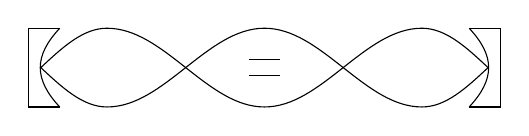
\begin{tikzpicture}[xscale=2]
                \draw (0, 1) -- (0, 0);
                \draw (0, 1) -- (0.2, 1);
                \draw (0, 0) -- (0.2, 0);
                \draw (0.2, 0) to [out=-245, in=245] (0.2, 1);

                \draw (3, 1) -- (3, 0);
                \draw (2.8, 1) -- (3, 1);
                \draw (2.8, 0) -- (3, 0);
                \draw (2.8, 0) to [out=-295, in=295] (2.8, 1);

                \draw (0.08, 0.5) sin (0.5, 1) cos (1, 0.5) sin (1.5, 0) cos (2, 0.5) sin (2.5, 1) cos (2.92, 0.5);

                \draw (0.08, 0.5) sin (0.5, 0) cos (1, 0.5) sin (1.5, 1) cos (2, 0.5) sin (2.5, 0) cos (2.92, 0.5);

                \draw (1.4, 0.4) -- (1.6, 0.4);
                \draw (1.4, 0.6) -- (1.6, 0.6);
        \end{tikzpicture}
\end{center}
Single cavity mode interacting with two level system in the RWA. Add coherent drive, dissipation via cavity loss $\kappa$ \& spontaneous emission rate $\gamma$
        \begin{block}{Interaction Hamiltonian}
                $\hat{\mathscr{H}} = \hbar \delta_{cd} \hat{a}^\dagger \hat{a} + \hbar \delta_{qd}\sigma_+ \sigma_- + \hbar g ( \hat{a} \sigma_+ + \hat{a}^\dagger \sigma_- ) + \hbar \xi (\hat{a} + \hat{a}^\dagger) $
        \end{block}
        \begin{block}{Master Equation}
                $\dot{\hat{\rho_S}} = \frac{i}{\hbar} [ \mathscr{H}, \rho_S] + \mathscr{L}_{\gamma} [\rho_S] + \mathscr{L}_{\kappa}[\rho_S]$
        \end{block}
\end{frame}
\begin{frame}
    \begin{block}{Resonant}
            $\delta_{cq} = \delta_{cd}=0$
            \footfullcite{Alsing1990}
            \footfullcite{Carmichael2015}
    \end{block}
\end{frame}
\begin{frame}
    \includegraphics[width=\linewidth, height=\textheight, keepaspectratio]{SPDSPslide.png}
\end{frame}
\begin{frame}
    \begin{block}{Dispersive}
            $\gamma \ll \kappa \ll g \ll \delta_{cq} \ll \omega_c$
            \footfullcite{Bishop2010}
    \end{block}
\end{frame}
\begin{frame}
    \includegraphics[width=\linewidth, height=\textheight, keepaspectratio]{DBslide.png}
\end{frame}
\printbibliography\
\end{document}
